\subsection{Cracking Minesweeper: Donald Knuth's version}

\renewcommand{\CURPATH}{equations/minesweeper_Knuth}

I first "invented" the method to crack minesweeper in early 2017.
Here is my first post and discussion:

\url{https://web.archive.org/web/20170306003313/https://yurichev.com/blog/minesweeper/}
\url{https://news.ycombinator.com/item?id=13797375}

Then I found almost the same method in Knuth's TAOCP Section 7.2.2.2, published in 2015, so he knew about it back then...

\begin{figure}[H]
\centering
\frame{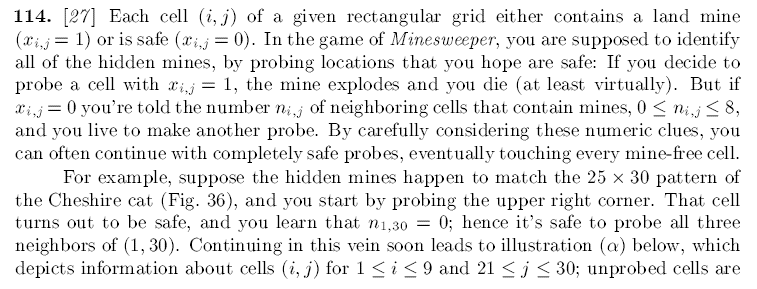
\includegraphics[scale=0.85]{\CURPATH/minesweeper1.png}}
\end{figure}

\begin{figure}[H]
\centering
\frame{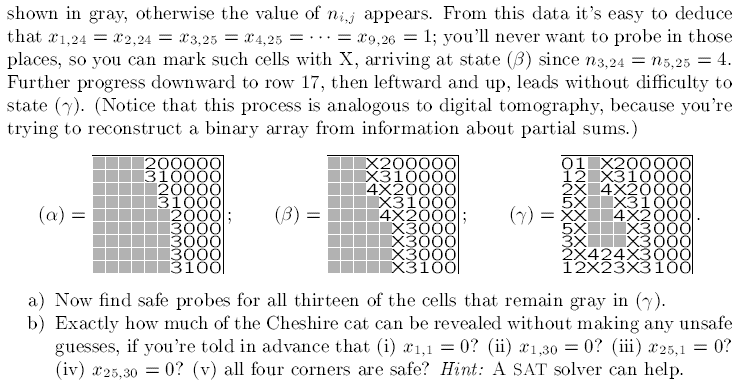
\includegraphics[scale=0.85]{\CURPATH/minesweeper2.png}}
\end{figure}

And solution:

\begin{figure}[H]
\centering
\frame{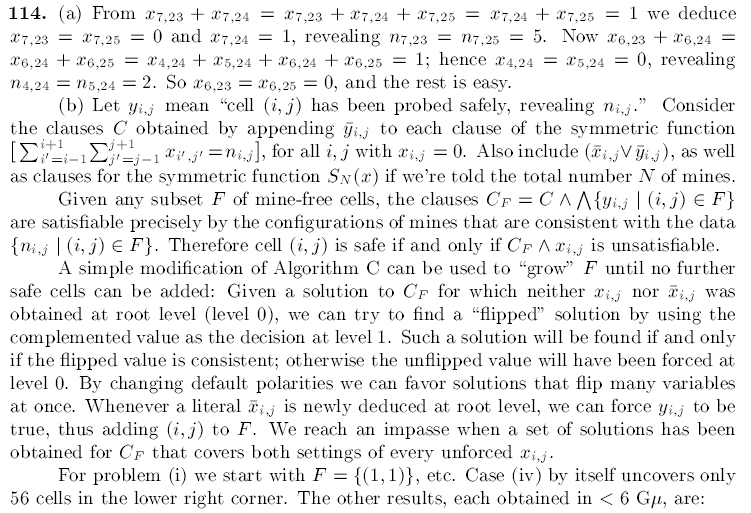
\includegraphics[scale=0.85]{\CURPATH/minesweeper3.png}}
\end{figure}

\begin{figure}[H]
\centering
\frame{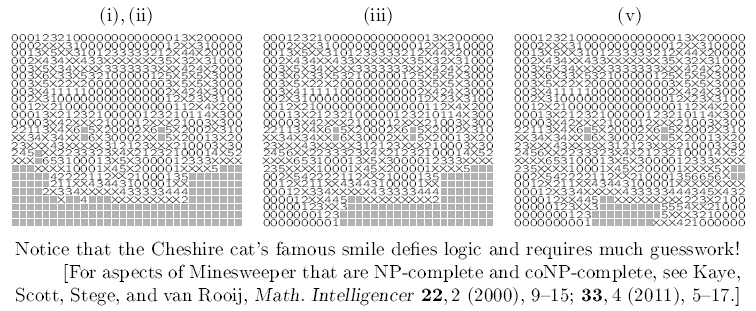
\includegraphics[scale=0.85]{\CURPATH/minesweeper4.png}}
\end{figure}
